\documentclass[12pt]{article}
\usepackage[a4paper, total={6.6in, 9.4in}]{geometry}

\setlength{\parskip}{3pt}

\usepackage{amsmath}
\usepackage{amssymb}
\usepackage{bm}
\usepackage{graphicx}
\usepackage{siunitx}
\usepackage{authblk}
\usepackage{url}
\usepackage{appendix}
\usepackage{booktabs}
\usepackage[font=small]{caption}
\usepackage{subcaption}

\usepackage [english]{babel}
\usepackage [autostyle, english = american]{csquotes}
\MakeOuterQuote{"}

\bibliographystyle{ieeetr}

\begin{document}

\title{Multi-phase classification of liquid crystal textures using convolutional neural networks}
\author{\textit{Joshua Heaton}\\\textit{10133722}}
\affil{Department of Physics and Astronomy, The University of Manchester}
\affil{MPhys project report}
\affil{Project performed in collaboration with James Harbon\\Supervisor: Dr Ingo Dierking}
\date{\today}

\maketitle

\begin{abstract}
\end{abstract}

\pagenumbering{gobble}
\newpage
\tableofcontents

\pagenumbering{gobble}
\newpage
\pagenumbering{arabic}

%~~~~~~~~~~~~~~~~~~~~~~~~~~~~~~~~~~~~~~~~~~~~~~~~~~~~~~~~~~~~~~~~~~~~~~~~~~~~~~~~~~~~~~~~~
\section{Introduction}
Machine learning (ML) is the term assigned to a wide range of computer algorithms that use data to automatically improve their performance on a specific task. These tasks can take various forms, including decision making, pattern recognition, and prediction  \cite{Murphy12}. A sub-field of ML known as deep learning (DL) generally consists of applying large-scale multi-layer neural networks, a type of algorithm inspired by the structure of the brain, to tasks involving highly complex abstractions of data. Such intensive algorithms typically require vast quantities of data and powerful computational resources to be trained effectively, with the advantage that they do not require any manual feature extraction \cite{Goodfellow16}. With the recent explosion in availability of such data and sophisticated computing technology, DL has seen a surge in interest and application among several fields \cite{Shrestha19}. Computer vision is one such field that has been impacted greatly. Convolutional neural networks (CNNs), a type of neural network suited particularly well to grid-based data, have proven extremely successful in the tasks of image classification, segmentation, and object detection \cite{Voulodimos18}.

There are many thousands of individual documented liquid crystal (LC) compounds, with each displaying a certain sequence of identifiable phases between that of a liquid and solid \cite{Dierking03}. Commonly, polarised microscopy is used to capture images of the textures produced by LC phases for identification by eye \cite{Dierking03}. Literature on machine learning for LC phase classification is sparse, with most studies focusing on the extraction of physical properties of LCs using simulated texture data \cite{Sigaki20, Sigaki19, Minor20, Walters19}, or other means \cite{Florin07, Butnariu13, Doi19, Inokuchi20}. Of most relevance is the work by Sigaki et al., in which they utilise CNNs to classify simulated isotropic and nematic phases to high accuracy \cite{Sigaki20}.

In this project, we prepare a novel dataset of LC texture images captured by polarised microscopy (PM), spanning multiple phases of all orders. Subsequently, we apply CNN classifier models to various phase groupings, probing the limits of attainable model accuracy. The work expands on and consolidates that of the first semester report \cite{Heaton20}, in which we demonstrated the viability of CNNs in some simple LC phase classification tasks. This report will provide a brief overview of LC phases, supervised ML, and neural networks, with further detail found in the first report \cite{Heaton20}. Details of the models used will then be provided, followed by a presentation of the results when they are applied to each of the prepared datasets. Summary conclusions and the limitations of the study will then be discussed.
%~~~~~~~~~~~~~~~~~~~~~~~~~~~~~~~~~~~~~~~~~~~~~~~~~~~~~~~~~~~~~~~~~~~~~~~~~~~~~~~~~~~~~~~~~
\section{Background principles}

\subsection{Liquid crystals}
Liquid crystal phases are characterised by the positional and orientational order of the molecular arrangement. In general, the phase of lyotropic LCs depends on the concentration of the sample in a solvent whilst thermotropic LCs, studied in this project, become more ordered with decreasing temperature. The order and overall structure of the LC phase determines its optical properties, in particular its birefringence. This enables images of the textures of a liquid crystal to be obtained by polarised microscopy, in which the sample is placed between two perpendicularly aligned polarisers. Polarised light incident on the set-up is altered in accordance with the current phase of the LC sample, producing characteristic features in the resulting image.

At sufficiently high temperatures, thermotropic LCs take the form of a fully anisotropic liquid with no structural order and hence birefringence, resulting in completely dark PM textures. Upon cooling, they will display at least one higher ordered phase before reaching the fully crystalline stage. Of lowest order, just orientational, is the nematic (N) phase, in which the molecules are aligned along a particular axis, called the director, and are still free to move around as in a liquid. Compounds with chiral molecules may instead display the cholesteric (N*) phase, which is the same as the nematic phase except with helical variation of the director. Layered positional order is introduced in the smectic phase, which is divided into three distinct phase groupings. The orientation of the director further categorises these groupings. The fluid smectic (FSm) phases have no positional order within molecular layers. The orientation of the director with respect to the layer planes determines whether the phase is smectic A (SmA), in which it is perpendicular, or C (SmC) otherwise. The smectic B (SmB), I (SmI), and F (SmF) phases are placed into the hexatic smectic (HSm) group, with short-range hexagonal structures generating positional order within the layers. The soft crystal phases differ in that the layers show long-range positional order.

This project uses CNNs to classify PM textures from thermotropic chiral LC compounds, including the phases N*, SmA, SmC, SmI, and SmF.  

\subsection{Supervised machine learning}
Machine learning algorithms can in general be categorised as supervised, unsupervised, or reinforcement learning. The ML implementations of this project are purely supervised learning algorithms. In this case, the ML model is defined as a function, parametrised by learned values $\bm{\theta}$, that maps an input data sample $\bm{x}$ containing various features to an output predicted label $\hat{\bm{y}}$,
\begin{equation}
\hat{\bm{y}}=f(\bm{x};\bm{\theta}). \label{supmodel} 
\end{equation}
$\hat{\bm{y}}$ can take various forms depending on the specific task, for example regression, in which the model attempts to predict a continuous value given the input data, or classification, in which it predicts a category that the input data sample belongs to. A supervised model attempts to learn appropriate $\bm{\theta}$ values for the mapping using a set of training data, consisting of pairs, $i$, of input examples and their corresponding true labels, $\lbrace\bm{x}^{(i)},\bm{y}^{(i)}\rbrace$. The model takes sample $\bm{x}^{(i)}$ and produces an output label prediction $\hat{\bm{y}}^{(i)}$ according to Equation \ref{supmodel}. A chosen cost function $J(\bm{y},\hat{\bm{y}};\bm{\theta})$ is then evaluated, which generally provides a measure of the divergence of the model outputs from the true labels. The parameters are then updated with a particular optimisation algorithm in order to minimise the cost. Successful training as such results in a model that is effective in producing accurate predictions for new unseen data samples. Fixed parameters that define the precise form of $f$, as well as training configurations, are known as hyperparameters.

When deciding on the form of a supervised model, of great importance is its capacity, which can be thought of as the size of the model. A low capacity model with few trainable parameters may not be able to extract or infer enough features from the training data to form good predictions, known as underfitting. On the other hand, too high a capacity will cause the model to learn meaningless or overly-fine features from the training data and it may not perform well when inferring on new unseen examples. This is referred to as overfitting. The model's hyperparameters must, therefore, be properly tuned to ensure it does not over or under fit. In addition to limiting model capacity, regularisation techniques can be applied to help prevent overfitting and improve generalisation.

Measurement of a supervised model's performance is critical in determining how well it will generalise to new unseen data, by evaluating a metric on a dataset of samples. As an example, for classification tasks a common metric is the percentage of samples that the model assigned to the correct class. Often, the training dataset is split into three subsets: training, validation, and test. The training set contains the data samples used to update the trainable parameters of the model. The validation set is used to tune the hyperparameters of the model. Evaluation of a trained model on the training and validation sets can reveal if the model has underfitted or overfitted. In the former case a low performance on both sets will be observed, whereas for the latter a high performance on the training set and low on the validation set will occur. Hyperparameters can then be adjusted accordingly before retraining the model. After a satisfactory model configuration and validation performance are reached, it is evaluated on the as-of-yet unseen test set to give an indication of the model's generalisation error.

\subsection{Neural networks}
\subsubsection{Layers}
Neural networks are a type of ML algorithm that pass input data through a series of layers, each containing a number of units. Every unit of a layer is connected in a particular way to the units of the previous layer. Units can take various forms including ones with or without trainable parameters, and specific layers are engineered so as to identify, manipulate, and propagate data features from the input to the output of the network. Perhaps the most simple type, in a dense layer the input to each unit is the outputs of all units of the previous layer. The inputs are multiplied by the unit's learned weight parameters and summed together with a learned bias parameter to calculate the unit's output. An activation function can then be applied to the output of each unit of the layer to introduce non-linearity to the network. Such non-linearities are essential in allowing a neural network to act as a universal function approximator, allowing it to perform highly complex inference on input data. A dense layer can hence be represented in matrix form as
\begin{equation}
\bm{O}=A(\bm{W}\bm{I}+\bm{B}), \label{dense}
\end{equation}
where $\bm{O}$ is the vector containing the outputs for the layer, $\bm{W}$ is the matrix of layer weights, $\bm{I}$ is the vector of layer inputs, $\bm{B}$ is the vector of bias parameters, and $A$ is the activation function applied element-wise.

Convolutional layers take grid-based input data such as two-dimensional images, and convolve it with a kernel of trainable parameters. The kernel has a width and height smaller than that of the input. The kernel is moved iteratively over the input, with the distance moved each iteration known as the stride of the convolution. At each step the kernel's parameters are multiplied with aligned input values, with the results summed together to produce the final output value. An activation function is often applied to this output value. The complete layer output is formed as a grid containing the ordered output values from the convolution. The size of the output grid depends on the dimensions of the kernel and the stride of the convolution, as these together determine the number of convolution steps in each direction. The input and output of the layer can have a third dimension, for example with the three colour channels of an RGB image. In this case, the kernel will have a different set of parameters for each channel. The number of channels can be increased from input to output by stacking the results from multiple kernels. A convolutional layer's padding refers to the behaviour of the kernel at the edges of the input. When the kernel is confined completely within the input space it is called valid padding. Same padding is when the kernel extends beyond the input space such that each value is visited by the kernel the same number of times, with kernel values outside the space multiplied by zero. For a stride of one in both directions, same padding will result in an output with the same shape as the input, and valid padding will result in dimensionality reduction.

The main advantage of convolutional layers over dense layers is the greatly reduced computational and memory cost, since they require far fewer parameters. The kernel parameters are shared over the entire input, which can also improve regularisation. Each kernel can be thought of as learning to extract a particular feature from the input to be passed on to the next layer, such as edges of objects in an image.

Pooling layers are often used after convolutional layers to reduce the dimensions of the network. They work in an analogous way to convolutional layers, however, the kernel has no trainable parameters to convolve and instead performs a specific operation. This could be, for example, taking the maximum value from the aligned input values at each step, known as max pooling. Average pooling takes the mean of the aligned input values. For pooling layers the kernel size is instead known as the pool size, and the pooling operation is applied to each input channel individually. Global pooling refers to the case in which the pool size is equal to the input size, which results in a vector output with one value for each of the input channels. Pooling layers are utilised to reduce the overall size and computational cost of the network whilst providing it with some invariance to translations of the input.

A common choice of activation function for dense and convolutional layers is the rectified linear unit (ReLU), defined as, for unit output $z$,
\begin{equation}
A(z)=\mathrm{max}(0, z), \label{relu}
\end{equation}
which is inspired by the behaviour of neurons in the brain. It has the advantage of introducing non-linearity without the potential for vanishing or exploding gradients when training the network. For classifier neural networks, the final output layer is a dense layer with a number of units equal to the number of classes. The softmax activation function is applied, which converts the output of each unit into a probability that the input sample belongs to the unit's corresponding class. For output unit $i$, this is defined as
\begin{equation}
\sigma(\bm{z})_i=\frac{e^{z_i}}{\sum_{j=1}^Ne^{z_j}}, \label{softmax}
\end{equation}
where $N$ is the total number of classes. The final output of the network is generally taken as the class with greatest assigned probability.

\subsubsection{Training}
Before training begins, a neural network's trainable parameters are randomly initialised from a particular distribution such as a normal distribution. A training step is performed by first selecting a "minibatch" containing a set number of random samples from the training set of data. The samples are passed through the network and a loss function is evaluated for each output. For classifier models, a widely used loss function, derived from the Kullback–Leibler divergence and maximum likelihood estimation, is the categorical cross-entropy, defined as
\begin{equation}
L(p)=-\mathrm{log}p
\end{equation}
where $p$ is the model's output probability that the sample belongs to the true labelled class. The cost function is then calculated as the average of the loss for all samples in the minibatch. An algorithm called backpropagation is then applied to calculate the gradient of the cost function with respect to the trainable parameters, $\bm{g}=\bm{\nabla}_{\theta}J(\bm{y},\hat{\bm{y}};\bm{\theta})$. Backpropagation, in summary, applies the chain rule of differentiation sequentially from the final network layer going backwards to the input layer, extracting the gradients at each unit output. A chosen optimisation algorithm is then applied to update the parameters, with a simple example being stochastic gradient descent. In this case, the parameters are updated against the gradient as
\begin{equation}
\bm{\theta}\leftarrow\bm{\theta}-\alpha\bm{g},
\end{equation}
where $\alpha$ is a hyperparameter called the learning rate, which modulates how much the parameters are adjusted with each step. This act of descending the cost function aims to reduce the loss when the model is evaluated on future samples, and in doing so improve its accuracy. Minibatches are sampled without replacement until the entire training set has been observed by the model, completing an epoch of training.

\subsubsection{Regularisation methods}
There are numerous methods of regularising neural networks in order to negate overfitting. Here the details are provided for methods utilised in this project.

Dataset augmentation aims to effectively increase the overall number of samples in the training set by performing transformations on the samples when they are selected for a minibatch, with the result taking the same label as the base sample. In the case of image data, alterations can be applied randomly and can include flipping the image, rotations, translations, and magnification within certain ranges. When used well, augmentations are a powerful and simple way to improve model generalisation.

Another simple yet highly effective regularisation method is early stopping. During training the model's performance on the validation set, usually simply the cost evaluated on the entire set, is recorded after every training epoch. Training stops if the cost has not decreased by more than a tolerance value after a certain number of epochs, defined by the patience hyperparameter. This helps greatly with regularisation because the model can overfit the training set if trained for too many epochs.

Dropout is a regularisation technique in which unit outputs in a layer are multiplied by zero with a set probability, called the dropout rate, with random units selected each training update step. This can viewed as training multiple sub-models with shared parameters, and it has the effect of reducing the neural network's sensitivity to noise.

For a layer with batch normalisation, after calculating the layer output values for each sample in a minibatch, the outputs are rescaled by subtracting the minibatch mean for each unit output and dividing by the standard deviation. The result for each unit is then rescaled linearly with extra learnable parameters. For output $z$ of a layer's unit this change is represented as
\begin{equation}
z\leftarrow\gamma\left(\frac{z-\mu}{\sigma}\right)+\beta, \label{batchnorm}
\end{equation}
where $\gamma$ and $\beta$ are the extra learnable parameters, $\mu$ is the mean and $\sigma$ is the standard deviation of the unit's output over the minibatch. For future computations on single samples, during training running averages of the means and standard deviations are recorded. Batch normalisation improves model stability whilst training and provides a regularising effect by introducing a form of noise.

%~~~~~~~~~~~~~~~~~~~~~~~~~~~~~~~~~~~~~~~~~~~~~~~~~~~~~~~~~~~~~~~~~~~~~~~~~~~~~~~~~~~~~~~~~
\section{CNN Models}
In this project we use three different types of CNN architectures, with each built from dense, convolutional, and pooling layers. All convolutional layers use a stride of $1\times1$, same padding, and ReLU activation, and all dense and convolutional layers have batch normalisation. A standard convolutional layer has kernel size $3\times3$, and a standard pooling layer refers to a max pooling layer with pool size and stride of $2\times2$ and same padding.

\subsection{Sequential}
The simplest models used are sequential CNNs. They consist of a series of standard convolutional layers, each followed by a standard pooling layer. The number of channels is doubled with each successive convolutional layer. The final convolutional layer in the network is followed instead by global average pooling, which is proceeded by two dense layers, first with a number of units equal to the number of channels in the previous convolutional layer, and second with half this. Both dense layers have ReLU activation and dropout rate 0.5. The final layer is the dense classification output with a number of units equal to the number of classes and a softmax activation. 

\subsection{Inception}
A set of models based on Google's Inception CNN architecture contain modules called inception blocks, which have parallel convolutional layers with different kernel sizes sharing inputs and outputs \cite{Szegedy15}. The structure of an inception block is detailed in Figure \ref{incblock}. 
\begin{figure}[!ht]
\centering
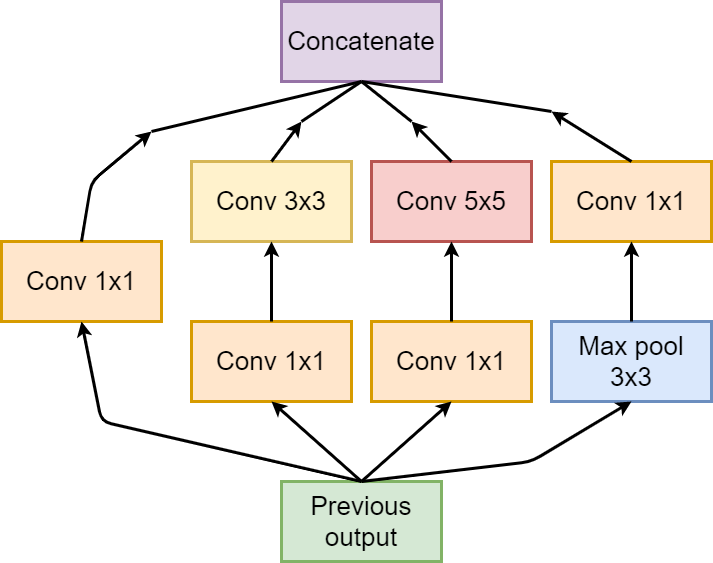
\includegraphics[width=4in]{images/inception_block.png}
\caption{Diagram of a single inception block, adapted from \cite{Szegedy15}. "Conv 1x1" represents a convolutional layer with kernel size $1\times1$ and "max pool 3x3" represents max pooling with pool size and stride of $3\times3$. The branching architecture with varying kernel sizes attempts to extract features of varying sizes from the input.}
\label{incblock}
\end{figure}
Our simplified inception networks begin with a convolutional layer with kernel size $7\times7$, followed sequentially by a standard pooling layer, a convolutional layer with kernel size $1\times1$, a standard convolutional layer, and a standard pooling layer. The output of this pooling layer is then fed into a series of one or more inception blocks. The output of the final inception block is followed sequentially by an average pooling layer with pool size and stride $5\times5$ and valid padding, a standard convolutional layer, and finally the same output dense layer structure as the sequential models starting with global average pooling. Similarly to the sequential models, the number of channels doubles with each convolutional layer, aside from inside the inception blocks, in which the number of channels is halved from the block input and then kept constant. The output concatenation has four times the channels as they are stacked from each branching layer. 

\subsection{ResNet}
The ResNet models, first implemented in 2015 by Kaiming He \textit{et al}., aim to tackle the problem of vanishing gradients in CNNs with many layers \cite{He15}. They do this by adding skip connections to the network, which feed the ouputs of layers early in the network to later layers, in conjunction with the standard sequential layer inputs. The specific model we utilise in this project is called ResNet50, owing to it having a total of 50 layers \cite{He15}. A diagram of architecture is presented in Figure .


%~~~~~~~~~~~~~~~~~~~~~~~~~~~~~~~~~~~~~~~~~~~~~~~~~~~~~~~~~~~~~~~~~~~~~~~~~~~~~~~~~~~~~~~~~
\section{Methodology}

\subsection{Data preparation}
All LC texture image data used has been obtained from polarised microscopy videos of LCs, labelled by compound and temperature range. If not provided, the phases displayed in the videos are identified using project supervisor Ingo Dierking's co-authored papers on homologous LC series \cite{Dierking94, Schacht95}. The software VLC Media Player \cite{VideoLan06} is used to extract image frames from the videos, and they are classified  according to the LC phase displayed at the point of extraction. The raw images have a resolution of $2048\times1088$. They are split into six smaller images of size $682\times544$ without compromising on the features displayed by each image. The images are then cropped to square $544\times544$ before being scaled down to the model input size of $256\times256$ and converted to greyscale with pixel value range [0, 1].

In construction of the training, validation, and test data sets, images of the same phase that also come from the same video are not divided between any of the three sets. This is to minimise potential data leakage, which is when samples in the training set are highly similar to samples in the validation or test sets, artificially inflating perceived model accuracy.

\subsection{Model training configurations}
We use the deep learning libraries TensorFlow and Keras to build and train all models \cite{Abadi16, Gulli17}. Model training is powered by NVIDIA CUDA, either on an NVIDIA RTX 2060 graphics card or cloud-based using Google Colaboratory \cite{Cook12, Bisong19}. All models are updated with the Adam optimiser, detailed in the first semester report, with variable learning rate and other fixed hyperparameter settings of $\beta_1=0.9$, $\beta_2=0.999$, and $\epsilon=10^{-7}$ \cite{Heaton20, Kingma14}. Early stopping is applied to all models, with a patience of 30 epochs and based on validation set cost. The final saved model parameters correspond to the epoch of training with the lowest validation set cost. Based on investigations of the previous semester, random flipping in both the horizontal and vertical directions are applied to the minibatches of images throughout training. These are the only augmentations used. Model accuracy is evaluated by the percentage of correctly classified images in the set. 

%~~~~~~~~~~~~~~~~~~~~~~~~~~~~~~~~~~~~~~~~~~~~~~~~~~~~~~~~~~~~~~~~~~~~~~~~~~~~~~~~~~~~~~~~~
\section{Summary of previous work}
The work of the first semester focussed on applying sequential, Inception and ResNet models to three different LC phase classification tasks. These included a four-phase set with isotropic, nematic, cholesteric, and smectic, a binary set with smectic A and C, and a general smectic set including fluid smectic, hexatic smectic, and soft crystal. The final models were trained three times each and the mean accuracy over all three runs calculated for the test sets. The error was calculated as half the range in accuracy. The results are summarised in Table \ref{sem1}.
\begin{table}[!htb]
\begin{center}
\caption{First semester mean test set percentage accuracies for final models and phase classification tasks.}
\begin{tabular}{l|c|c|c}
\toprule
& \textbf{Sequential} & \textbf{Inception} & \textbf{ResNet}\\
\midrule
\textbf{Four-phase} & $91\pm4\%$ & $0\pm0\%$ & $0\pm0\%$\\
\textbf{Smectic A and C} & $97\pm1\%$ & $97\pm2\%$ & $92\pm4\%$\\
\textbf{General smectic} & $86\pm6\%$ & $0\pm0\%$ & $0\pm0\%$\\
\bottomrule
\omit
\label{sem1}
\end{tabular}
\end{center}
\end{table}

%~~~~~~~~~~~~~~~~~~~~~~~~~~~~~~~~~~~~~~~~~~~~~~~~~~~~~~~~~~~~~~~~~~~~~~~~~~~~~~~~~~~~~~~~~
\section{Classification tasks and results}

\subsection{Cholesteric and smectic}

\subsection{Smectic A and C}

\subsection{Smectic I and F}

\subsection{Cholesteric, fluid smectic and hexatic smectic}

\subsection{Cholesteric, smectic A, C, I, and F}

%~~~~~~~~~~~~~~~~~~~~~~~~~~~~~~~~~~~~~~~~~~~~~~~~~~~~~~~~~~~~~~~~~~~~~~~~~~~~~~~~~~~~~~~~~
\section{Conclusions}

%~~~~~~~~~~~~~~~~~~~~~~~~~~~~~~~~~~~~~~~~~~~~~~~~~~~~~~~~~~~~~~~~~~~~~~~~~~~~~~~~~~~~~~~~~
\bibliography{report2}

\appendix
\appendixpage

\end{document}